% !TEX root = ../../../main.tex
% 来源：中学数学实验教材·第三册（高中数学）
% 章节：任意角的三角函数 / 三角函数的诱导公式
% 原始文件：6.tex，行 1221-1233
% 类型：tikz
% ---
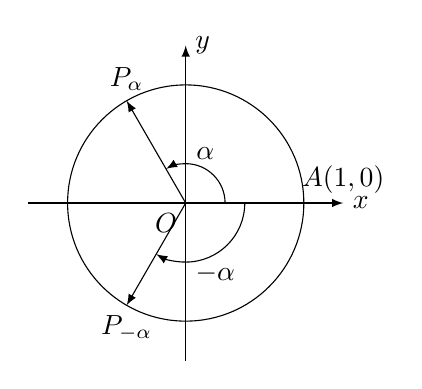
\begin{tikzpicture}[>=latex]
\draw[->] (-2,0)--(2,0)node[right]{$x$};
\draw[->] (0,-2)--(0,2)node[right]{$y$};
\draw (0,0) circle (1.5);
\draw[->](0,0)--(120:1.5)node[above]{$P_{\alpha}$};
\draw[->](0,0)--(-120:1.5)node[below]{$P_{-\alpha}$};
\draw[->] (.5,0) arc (0:120:.5);
\draw[->] (.75,0) arc (0:-120:.75);
\node at (60:.5)[above] {$\alpha$};
\node at (-60:.75)[below] {$-\alpha$};
\node at (2,0)[above]{$A(1,0)$};
\node at (-.25,-.25){$O$};
\end{tikzpicture}
